\section{Safety - A Method}
Risk, according to ISO 31000\cite{ISO31000}, is the effect of uncertainty on objectives. 
Therefore, in order to minimise risk we need to minimise uncertainty. 

In practical terms this means analysing the system from the top down,
creating a hierarchy of risks to ensure that all issues are considered. 
Taking this approach means that even if the engineer does not identify
every possible cause of failure (which is very likely), mitigation of the
failure modes not identified may still be achieved via global mitigations 
which are applied to an entire branch of the taxonomy. 
When applying a divide and conquer approach as shown in figure\ref{FailTree} we only need
to ensure that each failure set is equal to the union of those below it.

\begin{figure*}[!ht]
  \caption{A hierarchy of failures.}
  \label{FailTree}
  \centering
    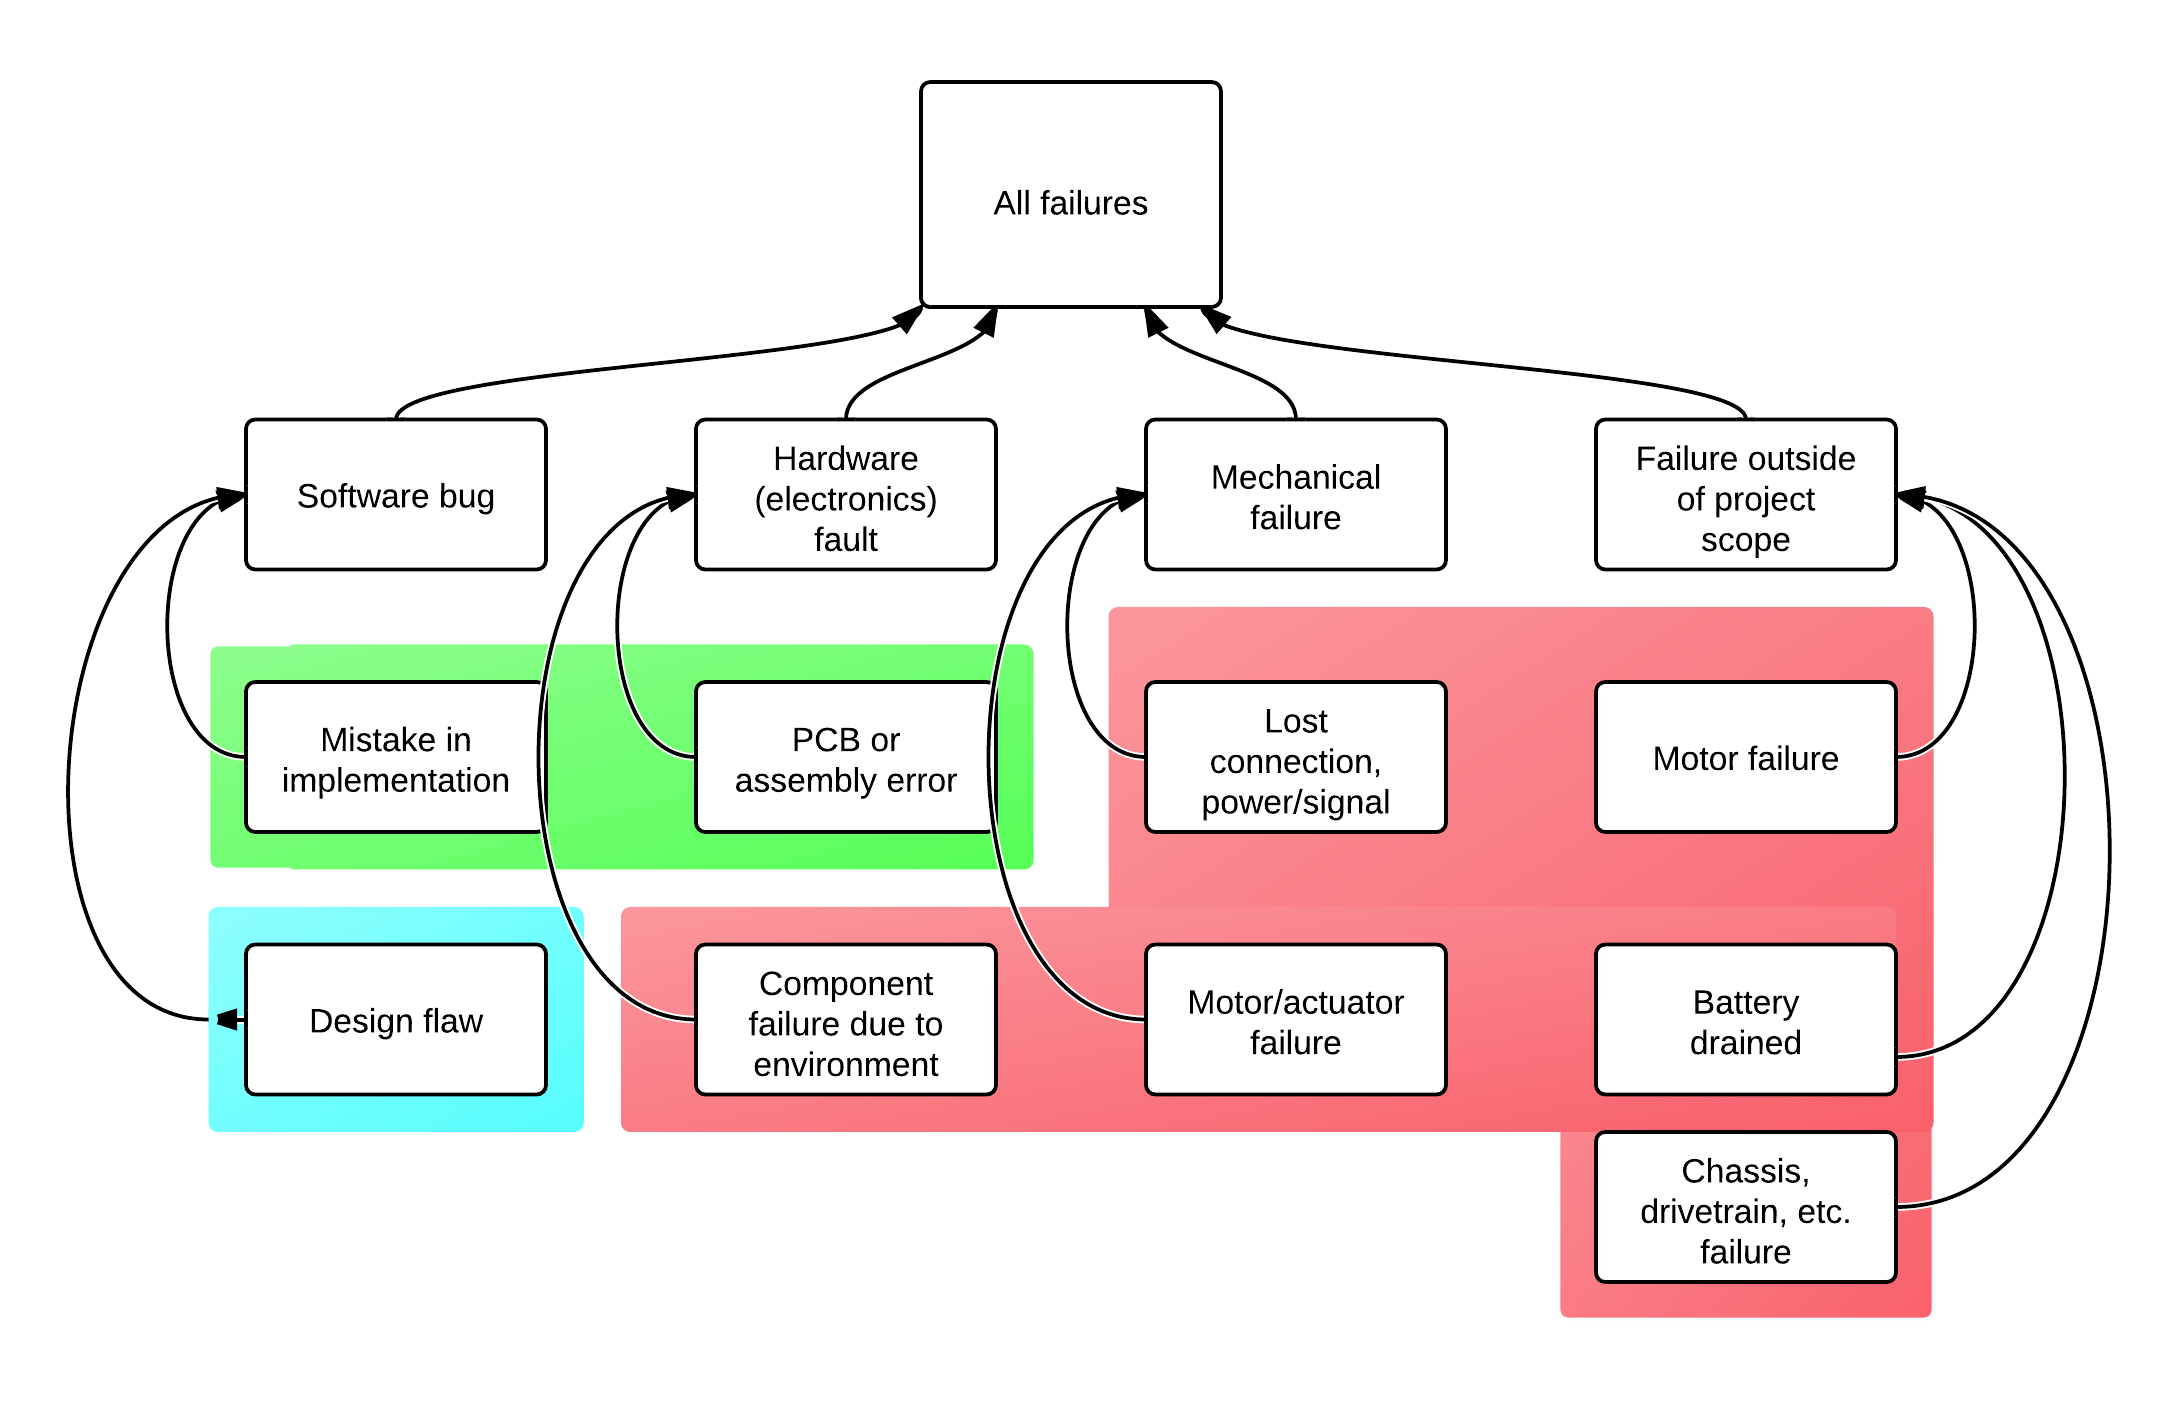
\includegraphics[width=\textwidth]{FailTree}
\end{figure*}

At the lowest level of figure\ref{FailTree} the categories are colour coded into the following groups:

\begin{itemize}
\item[G] Failures that are not a source of risk as they may be eliminated
during testing.
\item[R] Failures that are not preventable but may warrant mitigation.
\item[B] A failure which could happen unpredictably and could be more severe
than loss of power. Preventing this from occurring is the main focus of this paper.
\end{itemize}

\subsection{Preventing Mistakes (Green)}
For a detailed look into software and systems engineering practices see 
Looman's \emph{Software Engineering in the Mariokart System}\cite{
Looman_2011}. If standard design practices
such as unit testing are followed then it is possible to eliminate risk from these sources. 

\subsection{Risk Analysis (Red)}
Traditional project management tools for risk management involve tools
like Risk Matrices and qualitatively assessing the potential consequences and
probabilities of risks. Such tools are popular mainly for their simplicity
and have little backing in research, taking criticism from researchers such
as Tony Cox\cite{cox} for reasons such as their qualitative nature and reliance
on experienced judgement. Cox even goes as far to suggest that in some cases
using Risk Matrices leads to worse-than-random decisions.

For this reason and for simplicity's sake it was decided to lessen the consequences of
potential failure modes with a set of general mitigating techniques. Hence we have 
the following set of guidelines and design decisions:

\begin{itemize}
\item Despite the goal of autonomous function, a passenger should always be in
the vehicle during operation so that the vehicle may be shut down immediately 
by the provided kill switch.

\item All subsystems fall into an error state immediately after communication is
lost with any board. Any board losing then regaining power will also transition 
into an error state.

\item In the error state each board will perform whatever is necessary to minimise
the potential harm in case the go-kart is currently mobile. The important detail here
is that both the brake board and motor will attempt to slow the vehicle (the motor
is capable of regenerative braking) providing redundancy of the most critical function.

%%%%%%%%%%%%%% 
\end{itemize}
 


\subsection{Automated model checking to prevent design errors (Blue)}
While it is a given that a structural engineer will calculate forces and stress before
starting constructing and that a mechanical engineer may likewise simulate loads
on his or her design using a CAD package. Software engineering has,
due to the relative flexibility of the medium, been exempt from the expectation
 that a design must be proven before it is implemented. This is not 
 necessarily an advantage, however, as modelling can provide benefits
 including but not limited to proof of system robustness.

SPIN is an automated model checker for `the formal verification of
distributed software system.'\cite{spinroot} The name is an acronym for
Simple Promela INterpretor, where Promela is the language used to 
specify a model and its constraints. For more information on SPIN and
Promela visit spinroot.com but for the purposes of this paper an in-depth
knowledge is not required.

When modelling a software system, heavy-handed abstraction is useful
and sometimes necessary. This is because accurately modelling the software
to the level of calculations that have no effect on the system state only 
serves to increase the state-space and therefore the amount of computation
required to check the model. 

Conversely too much abstraction will limit the usefulness of a model to 
being little more than a way of sketching out the top level design of a 
distributed system.

Hence we wish to find an optimal level of detail  which will lie somewhere between the overly 
naive and ultimately useless model which assumes too much; and the result
of several years of work and many hours of computation which simulates
a system down to the instruction set level. 

The level of detail which is right for a project is subject to the law of diminishing
returns, where an increase in the severity of failure or the resources available to
the project will justify a more in depth model to be developed. 

\subsubsection{The (other) Benefits of Modelling a Distributed System}
The obvious aim of modelling is model checking, proving that a design is
correct. That is not the only benefit that modelling brings to a project
however. 

Writing a model before code provides the author with a `sketched' version of 
the code. Unlike a state diagram sketched on paper however the Promela
sketch can be simulated visually using the iSpin frontend for spin. iSpin
is capable of generating sequence diagram-like output showing message transmission
and reception between processes as well as other, more complicated graphical output 
we won't discuss here.

\subsection{Modelling Mariokart}
The software for mariokart was modelled with a focus on the state machine seen in 
appendix B and the message passing between boards. Failure was explicitly allowed
as seen in the first part of appendix A where the client board may non-deterministically
(the :: operator) choose to either reset itself, discover an error or continue running as
expected. Notice the probabilities of these three events occurring is not specified
as SPIN will exhaustively explore all possibilities regardless of their respective probabilities.

The constraints placed on the model enforce a consistent state between
the boards and ensure that the system either executes infinitely or all boards reach an 
error state and exit. Although the second option is not desirable in practice, showing
that the boards fail gracefully regardless of the failure mode is the most important
part of the model as it proves the correctness of an aspect of the system that would
be difficult or maybe even impossible to test manually.

As previously explained, if the team had more resources or if the
project came with significantly more danger (for example if the authors were modifying
a space shuttle instead of a go-kart) then a more in depth model would be justified.

As it stands, however, the time restrictions imposed on the project led to the relatively simple
model described above being developed quickly before being implemented in C.


\section{Discussion}
A responsible engineer evaluates his or her design before implementing it and it is the author's opinion 
that this belief is sometimes lacking in software development. Since a Promela model skips
the details of implementation it is simple to write and understand and does not bury the top level design 
in details. If written before implementation or concurrently it simplifies writing the actual software 
as the design is already specified and proven.

Balancing the cost of developing the model with the benefits it can bring is an important
consideration for any team wishing to travel the same path as the authors did with 
mariokart. For groups or individuals working on projects similar to the authors' it is recommended to
at least explore modelling top level designs before implementing them. The worst case outcome
is the cost of learning a new language (and Promela contains few difficult concepts) and the potential
benefits include quicker development times and the chance to catch a potentially dangerous fault
before it can manifest itself.

\section{Conclusion}
The potential for failure in the mariokart system was analysed. Solutions, mitigations and justifications
for ignoring potential problems were described along with the costs and benefits of modelling software. 
